% THIS IS SIGPROC-SP.TEX - VERSION 3.1
% WORKS WITH V3.2SP OF ACM_PROC_ARTICLE-SP.CLS
% APRIL 2009
%
% It is an example file showing how to use the 'acm_proc_article-sp.cls' V3.2SP
% LaTeX2e document class file for Conference Proceedings submissions.
% ----------------------------------------------------------------------------------------------------------------
% This .tex file (and associated .cls V3.2SP) *DOES NOT* produce:
%       1) The Permission Statement
%       2) The Conference (location) Info information
%       3) The Copyright Line with ACM data
%       4) Page numbering
% ---------------------------------------------------------------------------------------------------------------
% It is an example which *does* use the .bib file (from which the .bbl file
% is produced).
% REMEMBER HOWEVER: After having produced the .bbl file,
% and prior to final submission,
% you need to 'insert'  your .bbl file into your source .tex file so as to provide
% ONE 'self-contained' source file.
%
% Questions regarding SIGS should be sent to
% Adrienne Griscti ---> griscti@acm.org
%
% Questions/suggestions regarding the guidelines, .tex and .cls files, etc. to
% Gerald Murray ---> murray@hq.acm.org
%
% For tracking purposes - this is V3.1SP - APRIL 2009

\documentclass{acm_proc_article-sp}

\begin{document}

\title{Predicting the Feasibility of Potential Test Case Combinations}
\numberofauthors{2}
\author{
% 1st. author
\alignauthor
Bryan Robbins\\
       \affaddr{University of Maryland - College Park}\\
       \affaddr{Department of Computer Science}\\
       \affaddr{4115 AV Williams Building}\\
       \affaddr{College Park, MD 20742}\\
       \email{brobbins@cs.umd.edu}
% 2nd. author
\alignauthor
Atif Memon\\
       \affaddr{University of Maryland - College Park}\\
       \affaddr{Department of Computer Science}\\
       \affaddr{4115 AV Williams Building}\\
       \affaddr{College Park, MD 20742}\\
       \email{atif@cs.umd.edu}
}
\maketitle
\begin{abstract}
This is the abstract.
\end{abstract}

\category{D.2.5}{Software Engineering}{Testing and Debugging}
\terms{Experimentation, Verification}
\keywords{Software testing, model-based testing, test automation}

\section{Introduction}
Model-based software testing excels at the generation of short test cases. Often,
the collective group of test cases (called the test suite) provides a guarantee
of coverage. Consider various existing work by Memon et al., which generates test
cases for event-driven systems such as those driven by Graphical User Interfaces
(GUIs). Their sequence length coverage generation technique experiences an
exponential growth of possible test cases as longer sequence lengths are considered. This
growth often leads to a practical limit of considering only coverage of sequences 
of length 2 or 3 when generating test suites. Other research suggests that longer
test cases can more efficiently and more effectively find bugs than shorter test
cases.

In this paper, we lay the groundwork for constructing longer test cases from the shorter
test cases typical of model-based testing techniques. We explore whether shorter test cases
can be combined in interesting ways to produce longer test cases while still preserving
desired characteristics. As a first step, we consider the preservation of test case
feasibility. More precisely, we explore whether the execution results of model-based test
cases can be used to predict the feasibility of potential test case combinations. We believe
that this work can later be extended to the prediction of additional test suite properties,
and eventually to generalized reduction techniques for model-based test suites; but
we do not explore those extensions in this work.



\section{}

\section{The {\secit Body} of The Paper}

\begin{figure}
\centering
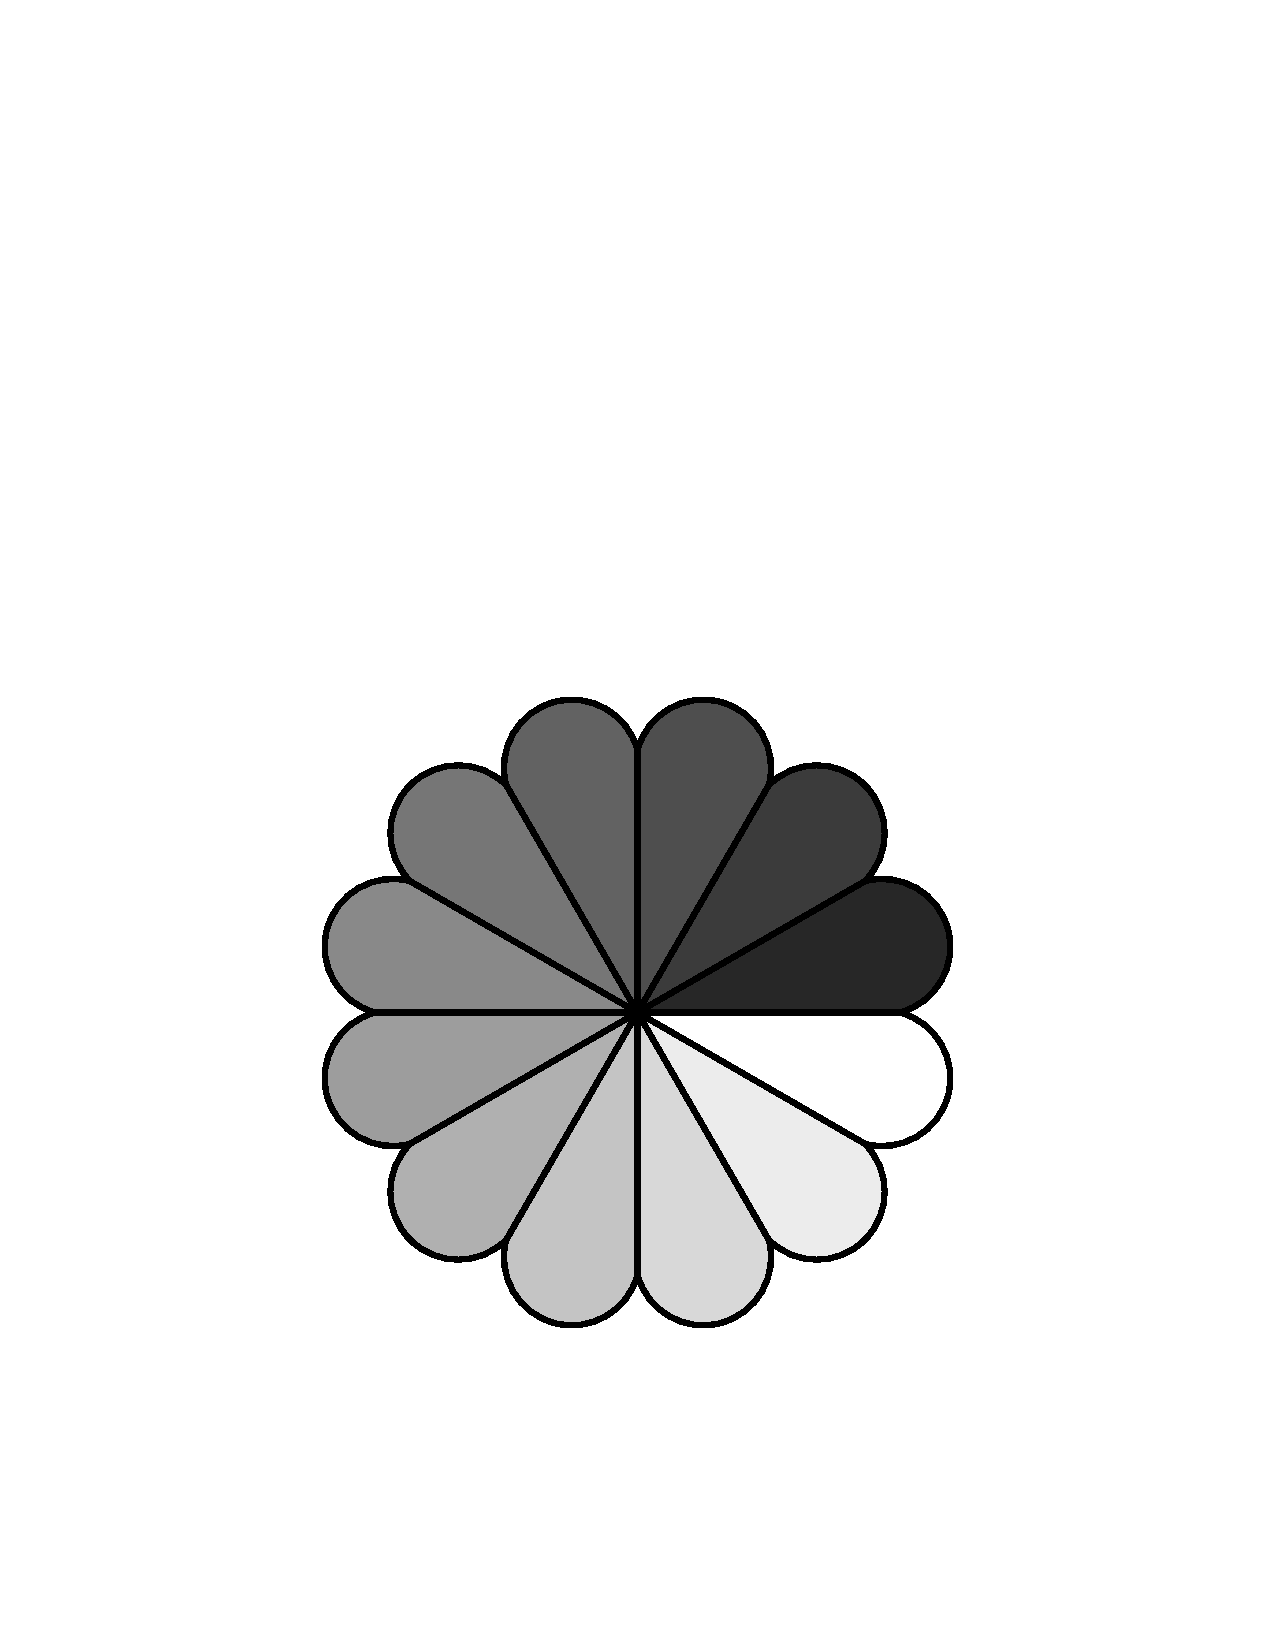
\includegraphics[height=1in, width=1in]{images/rosette.pdf}
\caption{Some Names I Know}
\end{figure}

\section{Conclusions}
This is the conclusion.


\bibliographystyle{abbrv}
\bibliography{amalga}
\balancecolumns
\end{document}
